\section{Practice Problems}
\begin{enumerate}
    \item Show that 
        \[V_0 = \frac12 (\frac{q}{\epsilon_s})(\frac{N_A N_D}{N_A + N_D}) W^2\]
    % \begin{Ans}
    %     We know that $\phi_{bi} = V_{th} \ln \left(\frac{N_A N_D}{n_i^2}\right) = \frac{kT}{q} \ln \left(\frac{N_A N_D}{n_i^2}\right)$
    % \end{Ans}
    \item Show that for a PN junction in which the $p$ side is much more heavily dped than the $n$ side (i.e. $N_A \gg N_D$) referred to as a $p^+ n$ diode. The following can be written as follows:
        \begin{align*}
            W &\simeq \sqrt{\frac{2 \epsilon_s}{q N_D}V_0}, ~~~~~ x_n \simeq W, ~~~~~ x_p \simeq \frac{W}{N_A / N_D} \\
            Q_j &\simeq A q N_D W, ~~~~~ Q_j \simeq A \sqrt{2 \epsilon_s q N_D V_0}
        \end{align*}
    
    \item For a Si PN junction that looks like this, where $N_A = 1 \times 10^{18}$ \conc and $N_D = 1 \times 10^{17}$ \conc. Given the built-in potential is 0. V and the relatively permittivity of Si is 12. No voltage is applied.
    \begin{figure}[htb]
        \centering
        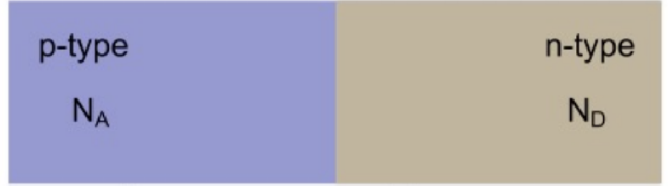
\includegraphics[scale=0.5]{figs/ch03/ans2.png}
    \end{figure}
    \begin{enumerate}
        \item Draw the charge along the horizontal axis.
        \item Draw the electric field along the horizontal axis. Label the critical points such as charge density, depletion width, and maximum electric field in your graphs.
    \end{enumerate}

    \item Considering a PN junction where the $n$ side is doped with $N_D = 10^{17}$ \conc and $p$ side is doped with $N_A = 10^{20}$ \conc, $n_i = 10^{10}$ \conc, kT/q = 26 mV, $\mu$n = 100 \mobility at $p$ side, $\mu$p = 400 \mobility at n side, L$_n$ = 2.3 \mun at $p$ side, and L$_p$ = 3.2 \mun at $n$ side, vacumn permittivity is $\epsilon_0 = 8.854 \times 10^{-12}$ C\sq/ (N $\cdot$ m\sq), the permittivity of silicon is 11.7$\epsilon_0$. Area of the PN junction is 1 \mun\sq
    \begin{enumerate}
        \item Calculate the built-in potential.
        \item Calculate the total depletion width at zero bias.
        \item Draw the electric field profile at zero bias (You need to calculate the maximum electric field). The left-hand side is N and the right-hand side is P.
        \item Calculate the depletion capacitance when the bias -1V. 
        \item Calculate the current when the bias is 1V.
        \item Find out the small-signal resistance and diffusion capacitance at 1V Given $\tau = 1 \mu$s. 
    \end{enumerate}
\end{enumerate}